\section{Allocation of time and resources}
\begin{comment}
SECTION NOT FINISHED. Here we are to write about what we think about following the wbs to structure our time. Was all the time spent with the supervisor and the customer optimal? Did we need all the resources given to us? Student assistant, group meetings with the class. Did we get the most out of our own group meetings or could we have done something different?
In the beginning, the team found the supervisors role somewhat confusing. After one or two meeting, and explicit asking the supervisor it became more clear to us that the supervisor was an overall support with focus on our report. And how we evaluated the risks throughout the project.
\end{comment}

This section presents an overview of the time and resource allocation in the project.

\subsection{Time allocation}
At the beginning of the project, the team did an estimation on how much time we would spend on each part of the project. In figure~\ref{fig:piechart} we show an overview on how much time we actually spent.

\begin{figure}[H]
\centering
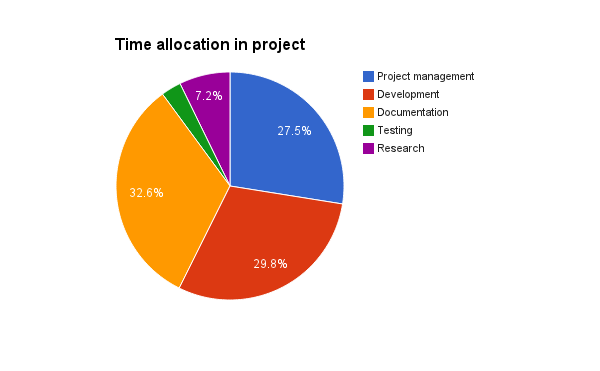
\includegraphics[width=0.6\textwidth, clip, trim=4cm 2cm 4cm 1cm]{ch/retrospect/fig/timePie.png}
\caption{Pie chart of time spent on different parts of the project.}
\label{fig:piechart}
\end{figure}

When comparing the actual time spent with the estimated time from table~\ref{tab:timeEstWP}, we see that the team spent more time on \todo[inline]{add more here when illustrations are ready}

\begin{figure}[H]
\centering
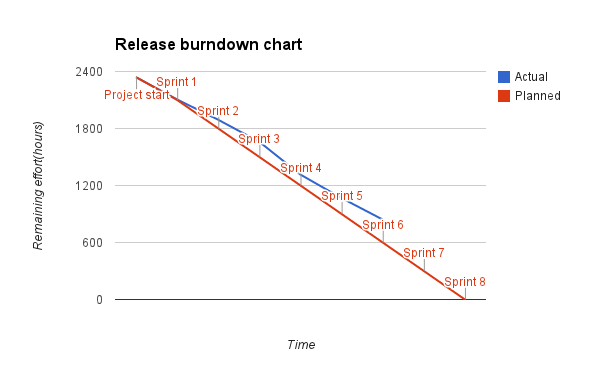
\includegraphics[width=0.7\textwidth, clip, trim=1.1cm 0.5cm 1.2cm 1cm]{ch/retrospect/fig/release.png}
\caption{Project release burn down chart}
\label{fig:release}
\end{figure}

\noindent In the release burn down chart, displayed in figure~\ref{fig:release}, we compare the estimated project progress with the progress we actually made. As the graph shows, the team worked less than the estimated number of hours. There are several reasons for this, including unplanned absence of team members, underestimation of tasks and too heavy workload due to deliveries in other subjects. Fortunately, the team had deliberately overestimated the number of work hours to compensate for lost time due to the school trip to China. This action resulted in that the team still was able to fulfill the course requirement and complete the assignment within the project's time scope.

\todo[inline]{oppdatere release og pie charten når sprint 7 og 8 er ferdig skrevet}

\subsection{Resource allocation}
